\documentclass[12pt, titlepage]{article}

\usepackage{amsmath}
\usepackage[margin = 1in]{geometry}
\usepackage{graphicx}
\usepackage{booktabs}
\usepackage{natbib}
\usepackage{array}

\usepackage{lipsum}
\usepackage[colorlinks=true, citecolor=blue]{hyperref}


\title{Association between Breast Cancer and Hepatitis C Virus with Age Confounding}
\author{Amy Traianou\\
  Department of Statistics\\
  University of Connecticut
}

\begin{document}
\maketitle


\begin{abstract}
The Kolmogorov--Smirnov (KS) test is one of the most popular goodness-of-fit
tests for comparing a sample with a hypothesized continuous distribution.
Nevertheless, it has often been misused.


\bigskip
\noindent{\sc Keywords}:
Breslow-Day;
Fisher's Exact Test;
Mantel-Haenszel.
\end{abstract}


\section{Introduction}
\label{sec:intro}

For this paper I decided to explore the risk factors associated with breast cancer in women. Breast cancer is extremely
prevalent and researchers are constantly trying to determine risk factors to identify women for preventative exams.
There are many studies attempting to determine if there is an association between certain risk factors and 
breast cancer including chronic hepatitis C infection \citep{Larrey2010is} and hepatitis B \citep{vishnu2016does}. 

Specifically, I want to determine if there is an association between testing positive for hepatitis C virus
and breast cancer. Both Hepatitis C and breast cancer are extremely prevalent in Egypt \citep{Hussein2021high}. 
Very recently on October 6th, Egypt and Qatar agreed to collaborate in the health sector and use each 
other's expertise. The health ministers specifically mentioned research in Hepatitis C and breast cancer
as a area of interest \citep{arham2022egypt}. Thus, research surrounding these diseases is becoming more
important in the field. 



\section{Data}
\label{sec:data}

The data I will be using is from a retrospective case control study conducted in 2020 \citep{2020association}. 
The data includes 405 subjects as part of the study group, all having been treated for breast cancer in the 
past 10 years. The second group consists of 145 adult females from a governorate in Egypt, who all participated 
in a cross-sectional study from 2015-2017. This data can be put into a 2x2 contingency table
for statistical analysis. 

\vspace{1cm}

2x2 Contingency Table for all patients.

\begin{tabular}{ | m{4cm} | m{4cm}| m{4cm} | m{2cm} | }
  \hline
    & HCV Seropositive & HCV Seronegative & Total\\ 
  \hline
  Breast Cancer & 88 & 317 & 405 \\ 
  \hline
  No Cancer Diagnosis & 15 & 130 & 145 \\ 
  \hline
  Total & 103 & 447 & 550 \\ 
  \hline
\end{tabular}

\vspace{1cm}

2x2 Contingency Table for pateints younger than 45.

\begin{tabular}{ | m{4cm} | m{4cm}| m{4cm} | m{2cm} | }
  \hline
    & HCV Seropositive & HCV Seronegative & Total\\ 
  \hline
  Breast Cancer & 17 & 110 & 127 \\ 
  \hline
  No Cancer Diagnosis & 2 & 91 & 93 \\ 
  \hline
  Total & 19 & 201 & 220 \\ 
  \hline
\end{tabular}

\vspace{1cm}

2x2 Contingency Table for patients older than 45.

\begin{tabular}{ | m{4cm} | m{4cm}| m{4cm} | m{2cm} | }
  \hline
    & HCV Seropositive & HCV Seronegative & Total\\ 
  \hline
  Breast Cancer & 71 & 207 & 278 \\ 
  \hline
  No Cancer Diagnosis & 13 & 39 & 52 \\ 
  \hline
  Total & 84 & 246 & 330 \\ 
  \hline
\end{tabular}

\section{Methods}
\label{sec:methods}

To test the association of breast cancer and Hepatitis C, I am going to use either the chi-square or Fisher's Exact test, depending on the
conditions from the sample size \citep{warner2013testing}. Fisher's exact test is useful for when the normality assumption is violated 
and the expected values of the 2x2 table are too small. The test uses the hypergeometric distribution to test if the probabilities are
the same between the two groups. Thus, we can determine if there is more of a risk of breast cancer for those with seropositive Hep C. As
 a result, we can determine if women who chronically test positive should be tested more frequently because they are at a higher risk. 
 
Figure~\ref{fig:formula} shows the probability of the original table occuring.

\begin{figure}[tbp]
  \centering
  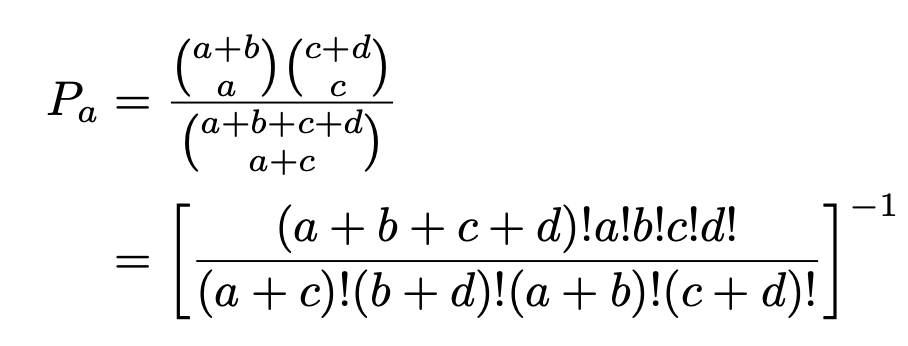
\includegraphics[width=8cm]{formula.png}
  \caption{Hypergeometric pmf.}
  \label{fig:formula}
\end{figure}


\section{Application}
\label{sec:app}

I expect to find an association between hepatitis C and breast cancer because there is some existing research that agrees with the association.
Therefore, this paper would corroborate the exisitng assumptions while giving them more of a basis. Although the potential impacts are quite 
minimal, the more research that supports the association, the better. If the investigation is not what I expect, then I would suggest more
data needs to be collected surrounding women with breast cancer in Eygpt. Specifically, a full prospective study with new samples. 


\section{Discussion}
\label{sec:discuss}

I expect to find an association between hepatitis C and breast cancer because there is some existing research that agrees with the association.
Therefore, this paper would corroborate the exisitng assumptions while giving them more of a basis. Although the potential impacts are quite 
minimal, the more research that supports the association, the better. If the investigation is not what I expect, then I would suggest more
data needs to be collected surrounding women with breast cancer in Eygpt. Specifically, a full prospective study with new samples. 


\bibliography{../manuscript/refs}
\bibliographystyle{chicago}

\end{document}
